\input{../header}
\usepackage{array}
\usepackage{amsmath}
\usepackage{tikz}
\usepackage{adjustbox}
\usepackage{xcolor}
\usepackage{tabto}
\usepackage[T1]{fontenc}
\usepackage{algorithm}
\usepackage{algpseudocode}
\newcolumntype{C}[1]{>{\centering\let\newline\\\arraybackslash\hspace{0pt}}m{#1}}


\usetikzlibrary{trees,positioning, shapes.multipart}


\newcommand{\vertcirc}{%
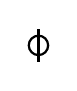
\begin{tikzpicture}[baseline=-0.5ex, line width=0.8pt]
  \draw (0,0) circle (0.35em);
  \draw (0,-0.6em) -- (0,0.6em);
\end{tikzpicture}%
}

\newcommand{\horcirc}{%
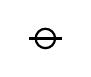
\begin{tikzpicture}[baseline=-0.5ex, line width=0.8pt]
  \draw (0,0) circle (0.35em);
  \draw (-0.6em,0) -- (0.6em,0);
\end{tikzpicture}%
}

\tikzset{
  bnode/.style={
    draw,
    rectangle split,
    rectangle split horizontal,
    rectangle split parts=2,
    text width=0.5cm, 
     align=center,
    minimum width=2cm,
    minimum height=0.8cm,
    inner sep=2pt,
    thick,
    font=\bfseries
  },
  level 1/.style={sibling distance=4cm, level distance=1.8cm},
  level 2/.style={sibling distance=2cm, level distance=1.8cm},
  level 3/.style={sibling distance=1.5cm, level distance=1.8cm},
  edge from parent/.style={
    draw,
    ->,
    thick
  }
}


\begin{document}

% Change the following values to true to show the solutions or/and the hints
\ShowSolutiontrue
\ShowWarningtrue
\ShowConseiltrue
\titre
\cours{Algorithmes spatiaux}

Le but de cette séance est de comprendre les caractéristiques des données spatiales et les structures de données couramment utilisées pour les manipuler. Lors de cette séance, nous implémenterons des algorithmes de manipulation de structures de données spatiales présentés en cours. Au terme de la séance, l'étudiant sera en mesure d'utiliser plusieurs algorithmes spatiaux pour résoudre des problèmes de base de façon efficiente.\\

\section{Nearest-Neighbor}
Dans cette section, nous allons implémenter une recherche du plus proche voisin. Le but de cette méthode est de trouver le voisin le plus proche du point de départ en tenant compte de ce point de ``départ" et un ensemble de points. Nous allons implémenter cet algorithme et ensuite l'étendre à un algorithme des ``k plus proches voisins'' (recherche des k voisins les plus proches plutôt que du seul voisin le plus proche). Les points seront représentés par des tuples construits manière suivante : point = (1,2) où 1 est l'abscisse et 2 l'ordonnée.\\
Nous vous recommandons de traiter les questions dans l'ordre.\\

\begin{Exercice}[5 minutes]\textbf{Python — La fonction de distance}\\

Pour implémenter notre recherche, nous avons besoin d'écrire une fonction permettant de calculer la distance entre 2 points. Ecrivez une fonction qui permet de calculer la distance entre 2 points.\\

\begin{conseil}
    Soit 2 points en 2 dimensions $({x_1},{y_1})$ et $({x_2},{y_2})$, la distance euclidienne entre ces 2 points est donnée par : $\sqrt{(x_2-x_1)^2+(y_2-y_1)^2}$. En Python, la fonction permettant de faire une racine carrée est \lstinline{sqrt} de la librairie \lstinline{math}. Pour mettre au carré, on utilise \lstinline{nombre\*\*2}.
\end{conseil}

\begin{solution}
   \lstinputlisting[language = python]{solutions/calculate_distance.py}
   Note: Vous pouvez utiliser \lstinline{**0.5} au lieu de la fonction \lstinline{math.sqrt()}.
\end{solution}
\end{Exercice}

\begin{Exercice}[10 minutes]\textbf{Python — Nearest-neighbor search}\\

Implémentez la recherche du voisin le plus proche. Cette dernière fonctionne de la façon suivante:
\begin{enumerate}
    \item Créez une fonction qui prend comme arguments une liste de points et un point de départ.
    \item Gérez le cas où la liste de points est vide.
    \item Traversez chaque point.
    \item Pour chaque point, calculez la distance entre ce point et le point de départ.
    \item Retournez un tuple contenant les coordonnées du point le plus proche sous forme d'un tuple et la distance — par exemple: $((x, y), dist)$.
\end{enumerate}
    
\begin{conseil}
    Utilisez la fonction de distance de la Question 1 et parcourez les points à l'aide d'une boucle \lstinline{for}. Si votre input est \lstinline{[(2, 3), (5, 6), (1, 4), (2, 4), (3, 5)]} et que le point de départ est \lstinline{(4, 4)}, alors l'output devra être \lstinline{((3, 5), 1.414)}. Ici, \lstinline{(3, 5)} sont les coordonnées du point le plus proche et \lstinline{1.414} est la distance euclidienne entre notre point de départ et le point le plus proche.  \\
    
    Note: Pour que votre programme fonctionne, écrivez votre algorithme du plus proche voisin dans le même programme que celui de la Question 1.
\end{conseil}
\begin{solution}
    \lstinputlisting[language = python]{solutions/nearest_neighbor.py}
\end{solution}
\end{Exercice}


\begin{Exercice}[15 minutes]\textbf{K-nearest-neighbor search}\\


Améliorez l'algorithme du voisin le plus proche effectué plus haut afin qu'il puisse retourner des \textit{K}-plus proches voisins.\\

\begin{conseil}
Appliquez l'algorithme du plus proche voisin \textit{K}-fois. À la fin de chaque itération, retirez le voisin le plus proche de l'ensemble des points sur lequel l'algorithme s'applique. De cette façon, vous trouverez le second voisin le plus proche, le troisième, etc...\\

Votre fonction devra retourner une liste sous la forme : $[(point1, distance1),(point2,distance2),...]$. En considérant un input \lstinline{[(2,3),(5,6),(1,4),(2,4),(3,5)]}, un point de départ \lstinline{(4,4)} et un nombre de voisins $K=2$, l'output de votre algorithme devra être : \lstinline{[((3, 5), 1.4142135623730951), ((2, 4), 2.0)]}. Attention au type des variables que vous manipulez. Pour rappel, les tuples sont immuables en Python. Pensez à créer de nouveaux tuples contenant les coordonnées des points et leurs distances.\\

Note : Pour que votre programme fonctionne, écrivez votre algorithme dans le même programme que celui de la Question 1 et la Question 2.
\end{conseil}

% \begin{solution}
%     \lstinputlisting[language = python, firstline=1, firstnumber=1, lastline=25]{solutions/Question3.py}
% \end{solution}
\begin{solution}
 \lstinputlisting[language = python, firstline=26, firstnumber=26]{solutions/K_nearest_neighbor.py}
\end{solution}
\end{Exercice}

\section{K-dimensional tree}

\begin{Exercice}[5 minutes]\textbf{Lecture du code — Construction d'un KD-Tree}

\begin{algorithm}
\caption{BuildKDTree($\text{points}, \text{depth}, k$)}
\label{alg:kdtree-build}
\begin{algorithmic}[1]
\If{$\text{points} = \emptyset$}
    \State \textbf{return} $\text{NIL}$
\EndIf
\State $\text{axis} \leftarrow \text{depth} \ \% \ k$ \Comment{Select axis based on current depth}
\State $\text{points} \leftarrow \text{SORT}(\text{points}, \text{key} = \text{axis})$ \Comment{Sort by current axis}
\State $\text{median\_idx} \leftarrow \text{INTEGER}(\text{length}(\text{points}) / 2 )$ \Comment{Index of median list item}
\State $\text{median} \leftarrow \text{KDNode}(\text{points}[\text{median\_idx}]$)
\State $\text{left} \leftarrow \text{points}[1 \ldots \text{median\_idx} - 1]$
\State $\text{right} \leftarrow \text{points}[\text{median\_idx} + 1 \ldots \text{length}(\text{points})]$
\State $\text{median.left} \leftarrow \text{BuildKDTree}(\text{left}, \text{depth} + 1, k)$
\State $\text{median.right} \leftarrow \text{BuildKDTree}(\text{right}, \text{depth} + 1, k)$
\State \textbf{return} median
\end{algorithmic}
\end{algorithm}

\begin{conseil}
Cet algorithme construit récursivement un arbre KD (KD-Tree) à partir d'une liste de points de dimension $k$. À chaque appel, il sélectionne d'abord l'axe de séparation en fonction de la profondeur courante (modulo le nombre de dimensions), puis trie les points selon cet axe et choisit le point médian comme racine du nœud courant afin de garantir un arbre équilibré. Les points situés avant ce médian constituent le sous-ensemble gauche et ceux après le médian le sous-ensemble droit. L'algorithme est appelé récursivement ensuite sur chacun de ces deux sous-ensembles pour construire respectivement les sous-arbres gauche et droit. Le processus se poursuit jusqu'à ce qu'il n'y ait plus de points à insérer.
\end{conseil}

\begin{solution}
Voir la démonstration des TP pour la visualisation de la construction d'un arbre KD.
\end{solution}

\end{Exercice}

\begin{Exercice}[10 minutes]\textbf{KD-Tree, un échauffement : Papier}\\
Vous trouverez ci-dessous une liste de points numérotés de 1 à 10. Placez-les dans un KD-Tree et dessinez la séparation de l'espace qui en résulte.

\begin{tikzpicture}[scale=0.30]

% --- style for coordinate labels ---
\tikzset{
    coordtext/.style={text opacity=0.45, opacity=0.45, font=\small}
}

% --- axes ---
\draw[->, thick] (-20,-18) -- (25,-18) node[right] {$x$};
\draw[->, thick] (-20,-18) -- (-20,12) node[above] {$y$};
\draw [dashed] (25,-18) -- (25,12);
\draw [dashed] (-20,12) -- (25,12);


% --- x ticks ---
\foreach \x in {-20,-15,-10,-5,0,5,10,15,20,25}
    \draw (\x,-18) -- (\x,-18.6) node[below] {\x};

% --- y ticks ---
\foreach \y in {-15,-10,-5,0,5,10}
    \draw (-20,\y) -- (-20.6,\y) node[left] {\y};

% --- points with labels ---
\node[circle, fill=black, inner sep=2pt, label=above:{A}] at (0,10) {};
\node[coordtext] at (0,10) [above right] {$(0,10)$};

\node[circle, fill=black, inner sep=2pt, label=right:{B}] at (-10,0) {};
\node[coordtext] at (-10,0) [right, xshift=0.5cm] {$(-10,0)$};


\node[circle, fill=black, inner sep=2pt, label=right:{C}] at (20,-5) {};
\node[coordtext] at (20,-5) [below left, xshift=-0.1cm] {$(20,-5)$};

\node[circle, fill=black, inner sep=2pt, label=right:{D}] at (-12,-7) {};
\node[coordtext] at (-12,-7) [below left] {$(-12,-7)$};

\node[circle, fill=black, inner sep=2pt, label=left:{E}]  at (-15,5)  {};
\node[coordtext] at (-15,5) [right, xshift=0.2cm] {$(-15,5)$};


\node[circle, fill=black, inner sep=2pt, label=right:{F}] at (0,6)   {};
\node[coordtext] at (0,6) [right, xshift=0.4cm] {$(0,6)$};

\node[circle, fill=black, inner sep=2pt, label=right:{G}] at (5,-6)  {};
\node[coordtext] at (5,-6) [right, xshift=0.5cm] {$(5,-6)$};


\node[circle, fill=black, inner sep=2pt, label=above:{H}] at (8,7)   {};
\node[coordtext] at (8,7) [above right, xshift=0.1cm] {$(8,7)$};

\node[circle, fill=black, inner sep=2pt, label=right:{I}] at (7,-15) {};
\node[coordtext] at (7,-15) [left] {$(7,-15)$};

\node[circle, fill=black, inner sep=2pt, label=right:{J}] at (15,4) {};
\node[coordtext] at (15,4) [right, xshift=0.4cm] {$(15,4)$};


\end{tikzpicture}

\begin{conseil}
La première division se fait de façon verticale. Veillez à bien insérer le point milieu (median) dans chaque étape. Les nœuds se situant au même niveau devraient diviser l'espace selon le même axe.
\end{conseil}

\begin{solution}
Voici le KD-Tree: 

\begin{center}
\adjustbox{margin=0.4cm}{
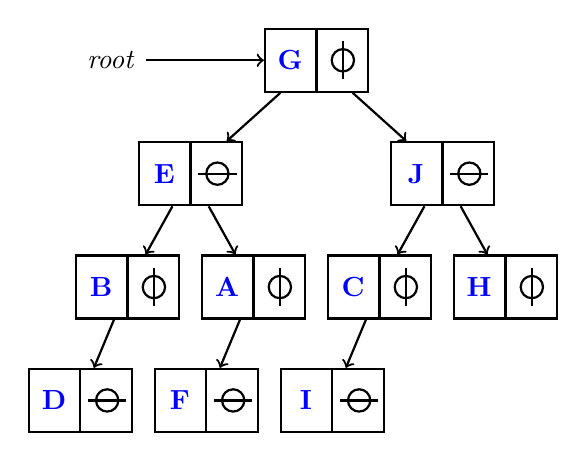
\begin{tikzpicture}[scale=0.8]
    % Tree
    \node[bnode] (n1) {\textcolor{blue}{G}\nodepart{two}{$\vertcirc$}}
        child { node[bnode] (n2) {\textcolor{blue}{E}\nodepart{two}{$\horcirc$}}
        child { node[bnode] (n4) {\textcolor{blue}{B}\nodepart{two}{$\vertcirc$}} 
            child { node[bnode] (n11) {\textcolor{blue}{D}\nodepart{two}{$\horcirc$}} }
            child[edge from parent path={}] {node { } }
        }
        child { node[bnode] (n5) {\textcolor{blue}{A}\nodepart{two}{$\vertcirc$}}
            child { node[bnode] (n6) {\textcolor{blue}{F}\nodepart{two}{$\horcirc$}} }
            child[edge from parent path={}] {node { } }
        }
        }
        child { node[bnode] (n3) {\textcolor{blue}{J}\nodepart{two}{$\horcirc$}}
        child { node[bnode] (n7) {\textcolor{blue}{C}\nodepart{two}{$\vertcirc$}}
            child { node[bnode] (n9) {\textcolor{blue}{I}\nodepart{two}{$\horcirc$}} }
            child[edge from parent path={}] { node { } }
        }
        child { node[bnode] (n8) {\textcolor{blue}{H}\nodepart{two}{$\vertcirc$}} }
    };

    % "root" label and arrow
    \node[left=1.5cm of n1] (rootlbl) {\textit{root}};
    \draw[->,thick] (rootlbl.east) -- (n1.west);
\end{tikzpicture}
}
\end{center}
La division de l'espace suivant le KD-Tree:

\centering
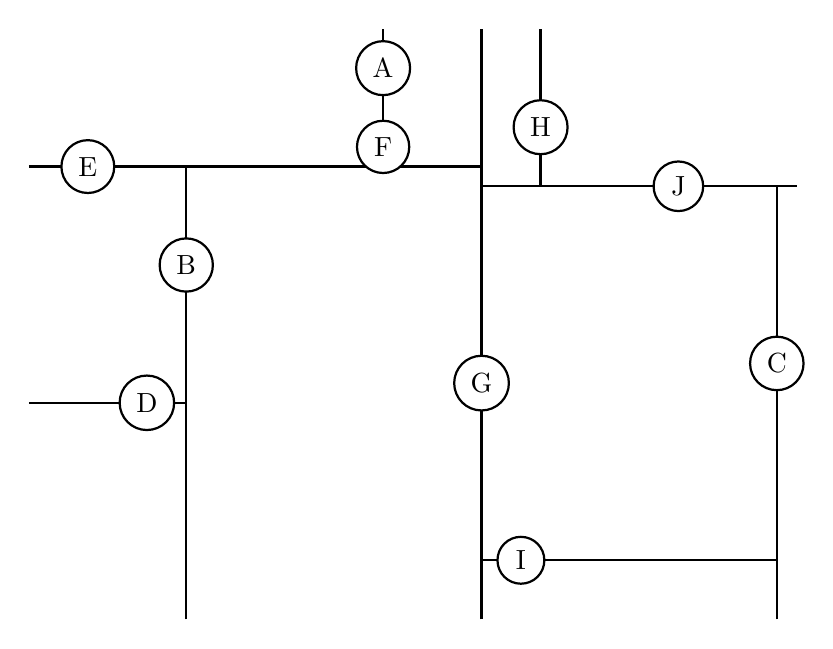
\begin{tikzpicture}[scale=0.25,
            dot/.style={
                circle,
                draw=black,
                fill=white,
                thick,
                minimum size=10pt
            }
        ]

        % % black line
        % \draw[black, thick] (0,-18) -- (0,12);
        % \draw[black, thick] (0,-5) -- (20,-5);
        % \draw[black, thick] (8,-5) -- (8,12);
        % \draw[black, thick] (8,4) -- (20,4);
        % \draw[black, thick] (5,-5) -- (5,-18);
        % \draw[black, thick] (5,-15) -- (20,-15);
        % \draw[black, thick] (0,0) -- (-18,0);
        % \draw[black, thick] (0,6) -- (-18,6);
        % \draw[black, thick] (-15,12) -- (-15,0);
        % \draw[black, thick] (-12,-18) -- (-12,0);
        
        \draw[black, thick] (5,-18) -- (5,12);
        \draw[black, thick] (-18,5) -- (5,5);
        \draw[black, thick] (5,4) -- (21,4);
        \draw[black, thick] (-10,-18) -- (-10,5);
        \draw[black, thick] (0,5) -- (0,12);
        \draw[black, thick] (-18,-7) -- (-10,-7);
        \draw[black, thick] (8,4) -- (8,12);
        \draw[black, thick] (20,-18) -- (20,4);
        \draw[black, thick] (5,-15) -- (20,-15);
        % \draw[black, thick] (0,-5) -- (20,-5);
        % \draw[black, thick] (8,-5) -- (8,12);
        % \draw[black, thick] (8,4) -- (20,4);
        % \draw[black, thick] (5,-5) -- (5,-18);
        % \draw[black, thick] (5,-15) -- (20,-15);
        % \draw[black, thick] (0,0) -- (-18,0);
        % \draw[black, thick] (0,6) -- (-18,6);
        % \draw[black, thick] (-15,12) -- (-15,0);
        % \draw[black, thick] (-12,-18) -- (-12,0);


        % circle on top of the line using the style
        \node[dot] at (0,10)   {A};
        \node[dot] at (-10,0)  {B};
        \node[dot] at (20,-5)  {C};
        \node[dot] at (-12,-7) {D};
        \node[dot] at (-15,5)  {E};
        \node[dot] at (0,6)    {F};
        \node[dot] at (5,-6)   {G};
        \node[dot] at (8,7)    {H};
        \node[dot] at (7,-15)  {I};
        \node[dot] at (15,4)   {J};

\end{tikzpicture}
\end{solution}
% \begin{tabular}{|c|}
% \hline
% \textbf{Graphe du KD-Tree} \\
% \hline
% \adjustbox{margin=0.4cm}{
% \begin{tikzpicture}[scale=0.8]
%     % Tree
%     \node[bnode] (n1) {\textcolor{blue}{A}\nodepart{two}{$\vertcirc$}}
%         child { node[bnode] (n2) {\textcolor{blue}{B}\nodepart{two}{$\horcirc$}}
%         child { node[bnode] (n4) {\textcolor{blue}{D}\nodepart{two}{$\vertcirc$}} }
%         child { node[bnode] (n5) {\textcolor{blue}{E}\nodepart{two}{$\vertcirc$}}
%             child[edge from parent path={}] {node { } }
%             child { node[bnode] (n6) {\textcolor{blue}{F}\nodepart{two}{$\horcirc$}} }
%         }
%         }
%         child { node[bnode] (n3) {\textcolor{blue}{C}\nodepart{two}{$\horcirc$}}
%         child { node[bnode] (n7) {\textcolor{blue}{G}\nodepart{two}{$\vertcirc$}}
%             child[edge from parent path={}] { node { } }
%             child { node[bnode] (n9) {\textcolor{blue}{I}\nodepart{two}{$\horcirc$}} }
%         }
%         child { node[bnode] (n8) {\textcolor{blue}{H}\nodepart{two}{$\vertcirc$}}
%             child[edge from parent path={}] { node { } }
%             child { node[bnode] (n10) {\textcolor{blue}{J}\nodepart{two}{$\horcirc$}} }
%         }
%     };

%     % "root" label and arrow
%     \node[left=1.5cm of n1] (rootlbl) {\textit{root}};
%     \draw[->,thick] (rootlbl.east) -- (n1.west);

% \end{tikzpicture}
% }
% \\
% \hline
% \textbf{Division de l'espace suivant le KD-Tree} \\
% \hline
% \adjustbox{margin=0.6cm}{
% \begin{tikzpicture}[scale=0.29,
%             dot/.style={
%                 circle,
%                 draw=black,
%                 fill=white,
%                 thick,
%                 minimum size=10pt
%             }
%         ]

%         % black line
%         \draw[black, thick] (0,-18) -- (0,12);
%         \draw[black, thick] (0,-5) -- (20,-5);
%         \draw[black, thick] (8,-5) -- (8,12);
%         \draw[black, thick] (8,4) -- (20,4);
%         \draw[black, thick] (5,-5) -- (5,-18);
%         \draw[black, thick] (5,-15) -- (20,-15);
%         \draw[black, thick] (0,0) -- (-18,0);
%         \draw[black, thick] (0,6) -- (-18,6);
%         \draw[black, thick] (-15,12) -- (-15,0);
%         \draw[black, thick] (-12,-18) -- (-12,0);


%         % circle on top of the line using the style
%         \node[dot] at (0,10)   {A};
%         \node[dot] at (-10,0)  {B};
%         \node[dot] at (20,-5)  {C};
%         \node[dot] at (-12,-7) {D};
%         \node[dot] at (-15,5)  {E};
%         \node[dot] at (0,6)    {F};
%         \node[dot] at (5,-6)   {G};
%         \node[dot] at (8,7)    {H};
%         \node[dot] at (7,-15)  {I};
%         \node[dot] at (15,4)   {J};

% \end{tikzpicture}
% }
% \\
% \hline
% \end{tabular}
% \end{solution}

\end{Exercice}


\begin{Exercice}[15 minutes]\textbf{KD-Tree : Python}\\

L'objectif de cet exercice est d'écrire une fonction permettant d'ajouter un nœud à un KD-Tree. Les nœuds sont sous la forme $[(x,y)$, enfant à gauche, enfant à droite$]$, $x$ et $y$ étant les coordonnées du nœud considéré. Chaque enfant peut être soit un nœud ou une feuille. Complétez le code contenu dans le fichier \lstinline{Question6.py}. \newline 

Voici le pseudo-code permettant d'ajouter un nœud à un KD-Tree:
    \begin{algorithm}[H]
        \caption{AddKDTree($\text{node}, \text{point}, k, \text{cutaxis}$)}
    \begin{algorithmic}[1]
    \If{$\text{node} = \text{NIL}$}
        \State $\text{new\_node} \leftarrow \text{KDNode}(\text{point})$    \State \textbf{return} $\text{new\_node}$
    \EndIf
    \If{$\text{point}[\text{cutaxis}] \leq \text{node}.\text{point}[\text{cutaxis}]$} \Comment{Insert into the left (lesser) subtree}
        \State $\text{new\_cutaxis} \leftarrow (\text{cutaxis} + 1) \pmod k$
        \State $\text{node}.\text{left} \leftarrow \text{AddKDTree}(\text{node}.\text{left}, \text{point}, k, \text{new\_cutaxis})$
    \Else
        \State $\text{new\_cutaxis} \leftarrow (\text{cutaxis} + 1) \pmod k$
        \State $\text{node}.\text{right} \leftarrow \text{AddKDTree}(\text{node}.\text{right}, \text{point}, k, \text{new\_cutaxis})$
    \EndIf
    \State \textbf{return} $\text{node}$
    \end{algorithmic}
    \end{algorithm}
\begin{attention}
Afin de simplifier la question, vous ne devez pas créer une classe \texttt{KDNode} pour représenter les nœuds. Chaque nœud est représenté comme une liste. Donc, quand vous transformez le pseudocode, \texttt{node.point} sera \texttt{node[0]}, \texttt{node.left} sera \texttt{node[1]}, et \texttt{node.right} sera \texttt{node[2]}.
\end{attention}
\begin{conseil}    
    Si votre réponse est correcte, votre programme devrait afficher : \lstinline{[(0, 10), [(-10, 0), None, None], None]}. Pour rappel, en Python, \lstinline{NIL} correspond à \lstinline{None}. Dans le pseudocode, \lstinline{KDNode} permet de créer un nouveau nœud. Vous pouvez vous inspirer de la structure de \lstinline{main} définie dans le fichier \lstinline{Question6.py}.
\end{conseil}

\begin{solution}
\lstinputlisting[language = python, firstline=1, firstnumber=1, lastline=17]{solutions/KD_add_node.py}
\end{solution}
\begin{solution}
\lstinputlisting[language = python, firstline=19, firstnumber=19]{solutions/KD_add_node.py}
\end{solution}
\begin{solution}
Si la coordonnée du point à ajouter est inférieure à celle du nœud selon l'axe de découpe en considération, alors le point doit se trouver dans le sous-arbre de gauche. Par convention, le nœud de gauche correspond dans la liste [(x,y), nœud de gauche, nœud de droite] à l'indice 1, par conséquent, on appelle la fonction de façon récursive pour ajouter le point, mais cette fois-ci en partant d'un cran plus bas dans l'arbre. Cela se répète jusqu'à ce qu'on ait atteint les feuilles et qu'un nouveau nœud doive être créé.
\end{solution}
\end{Exercice}

\section{ Quad-Tree}
\begin{Exercice}[10 minutes]\textbf{Une mise en train : Papier}\\

Encodez les images ci-dessous dans un Quad-Tree.\\

\begin{table}[h!]
\centering
\begin{tabular}{|c|c|}
\hline
\textbf{Image 1} & \textbf{Image 2} \\
\hline
\adjustbox{margin=0.3cm}{

\includegraphics[]{resources/Quad-Tree 1.PNG}
}
&
\adjustbox{margin=0.3cm}{

\includegraphics[]{resources/Quad-Tree 2.PNG}
}
\\
\hline
\end{tabular}
\end{table}

\begin{conseil}
   Pour réussir cet exercice vous devez diviser chaque nœud en 4 sous-espaces (le plus petit sous-espace étant un carré) de taille égale, et ce autant de fois que nécessaire. La branche la plus à gauche (en haut) correspond au quadrant \lstinline{NW} puis en allant de gauche à droite et puis en bas (comme dans le sens de lecture): \lstinline{NE, SW, SE}. \\
    
    \textbf{Indice :} Votre arbre devrait avoir une profondeur de 2 et disposer de 16 feuilles.
\end{conseil}
\begin{solution}
Image 1 :\\
    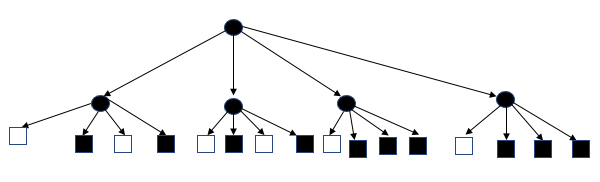
\includegraphics[scale=0.65]{solutions/Quad-Tree 1 solution.PNG}\\
    
Image 2: \\
    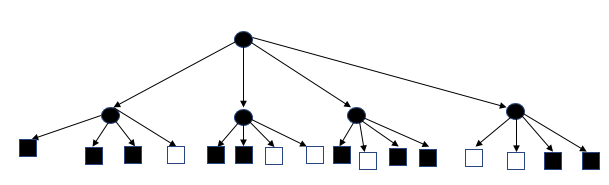
\includegraphics[scale=0.65]{solutions/Quad-Tree 2 solution.PNG}
\end{solution}
\end{Exercice}
\begin{Exercice}[10 minutes]\textbf{Une mission capitale : Papier \optionnel}\\

Récemment embauché par la CIA, vous êtes à la recherche d'un individu se cachant dans une des villes suivantes : Bleu, Orange, Noir, Gris, Vert et Jaune. Votre mission, si vous l'acceptez, est de créer un Quad-Tree qui vous permettra de géolocaliser le criminel de façon efficace. Vous trouverez ci-dessous une carte de villes. Créez le Quad-Tree et rétablissez la justice.\\

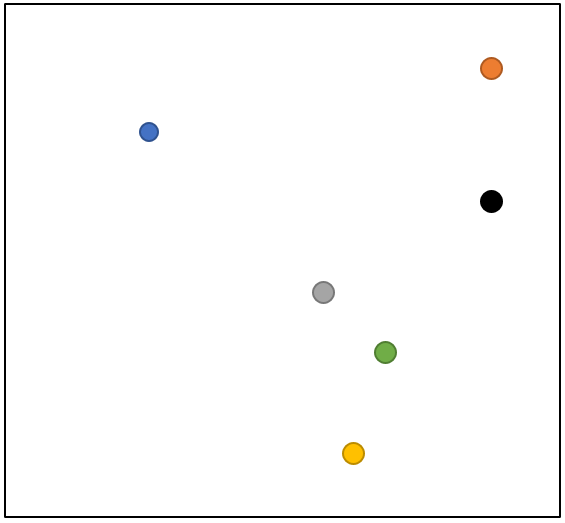
\includegraphics[]{resources/Quad-Tree 3.PNG}
\begin{conseil}
    Commencez par diviser la carte de la ville de façon adéquate puis construisez le graphe.\\
    
    \textbf{Remarque: }Les différentes branches de l'arbre n'auront pas toutes la même profondeur.
\end{conseil}
\begin{solution}
    Voici la division de la carte qui permet de construire le Quad-Tree :\\
    
    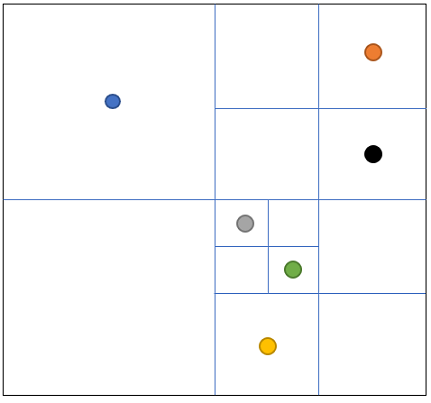
\includegraphics[]{solutions/Quad-Tree 3 solution 1.PNG}\\
    
    Le Quad-Tree qui en résulte :\\
    
    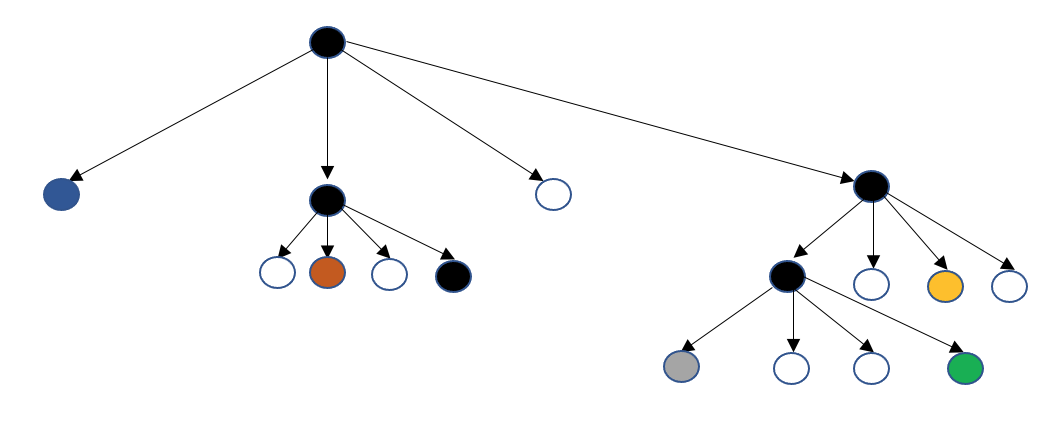
\includegraphics[scale=0.65]{solutions/Quad-Tree 3 solution 2.1.png}\\
    
    Note : Un rond blanc correspond à un quadrant vide.
    
\end{solution}
\end{Exercice}

\end{document}
